

 In this section we empirically investigate the effect that the receptive field has in a network's trainability and
 prunability. We Statistically validate our results on VGG and ReseNet50 architecture and in CIFAR10 and Tiny ImageNet
 datasets. 


 \todo[inline]{Here I never talked of how I calculated the receptive field, which I used a libary that calculates
 the gradient projection in a dummy input space with a projected gradient of 1 in the middle of all the fueature maps of the
last convolutional layer for the two architectures.
}


\subsection{Experimental settings}
We used a custom implementation of the ResNet50 and VGG models with a modified maxpooling layer after the first
convolutional layer for manipulating the receptive field. Implementation details are in \Cref{subsec:
implementation_details}. The dataset are CIFAR10 and Tiny ImageNet. The training hyperparameters are the following:
\begin{itemize}
  \setlength\itemsep{.0em}
    \item Epochs: 200
    \item Optimizer: SGD
    \item Learning rate: 0.0001
    \item Learning rate schedule: Cosine annealing with $T_{max}=200$ 
    \item Momentum: 0.9
    \item Weight Decay: $5 \times 10^{-5}$
    \item Gradient clipping: 0.1
\end{itemize}


\subsection{Manipulating the Receptive Field}

There is plentiful of ways for Manipulating the receptive field. It is known that the presence of skip connections
affect the receptive fields along with depth and dilation on convolutions. We wanted to alter the receptive field
minimum alterations to the rest of the networks leaving all layers with the exact same number of parameters. We placed a
maxpooling layer just after the first convolutional layer on both architectures and we changed the kernel size of that
layer. That is the only difference between the different models on each experiment. For each
architecture-dataset-receptive field combination we trained 5 models and the result are shown in \ref{sec:rfanda}.
\subsection{Receptive Field, Accuracy and Loss Landscape}
\label{sec:rfanda}
Here we show the dense accuracy after training the models and its one-shot pruned accuracy. One interesting observation
is that larger receptive field correlates with lower accuracy but simultaneously its one-shot pruning performances is
better than those for smaller receptive fields. This behaviour generalises across all the combinations of
architecture-dataset. In \Cref{subsec:OneShotPruningrates} we show that the current trend in accuracy (for dense and prune version) only
arises for sufficiently large pruning rate (>0.8). We also fine-tuned the models to test their real-world application
capabilities as seen  in \Cref{subsec:Fine_tuning_solutions} but here we only show the pruning rate of 0.9 as means to
show the one-shot behaviour of these networks in order to understand their one-shot potential.
For each one of the combinations shown here we trained and pruned 5 models, the values presented are the mean  with its
standard deviation.

The image size for CIFAR10 and Tiny ImageNet is 32x32 and  64x64 respectively. In both cases the receptive fields of
each architecture is greater than the size of the image.

% Please add the following required packages to your document preamble:
% \usepackage{booktabs}
\begin{table}[H]
\begin{tabular}{@{}cccc@{}}
\toprule
\multicolumn{4}{c}{\textbf{VGG}}                                                                                                                                                                          \\ \midrule
\multicolumn{1}{l}{\textbf{Receptive Field}} & \multicolumn{1}{l}{\textbf{Dense Test Accuracy}} & \multicolumn{1}{l}{\textbf{Pruned Test Accuracy}} & \multicolumn{1}{l}{\textbf{Difference in Accuracy}} \\
181                                          & 93.5 $\pm$ 0.11                                  & 10.9 $\pm$2.03                                    & 82.6 $\pm$ 2.02                                     \\
359                                          & 91.1 $\pm$ 0.23                                  & 32.4 $\pm$ 15.7                                   & 58.7 $\pm$ 15.8                                     \\
537                                          & 87.8 $\pm$ 0.19                                  & 87.6 $\pm$ 0.30                                   & 0.18 $\pm$ 0.16                                     \\
715                                          & 85.8 $\pm$ 0.21                                  & 85.8 $\pm$ 0.22                                   & 0.07 $\pm$ 0.04                                     \\ \midrule
\multicolumn{4}{c}{\textbf{Resnet 50}}                                                                                                                                                                    \\ \midrule
\multicolumn{1}{l}{\textbf{Receptive Field}} & \multicolumn{1}{l}{\textbf{Dense Test Accuracy}} & \multicolumn{1}{l}{\textbf{Pruned Test Accuracy}} & \multicolumn{1}{l}{\textbf{Difference in Accuracy}} \\
110                                          & 94.8 $\pm$ 0.29                                  & 56 $\pm$ 20.7                                     & 38.7 $\pm$ 20.5                                     \\
213                                          & 94.0 $\pm$ 0.16                                  & 91.7 $\pm$ 0.98                                   & 2.25 $\pm$ 0.90                                     \\
318                                          & 92.2 $\pm$ 0.18                                  & 91.4 $\pm$ 0.45                                   & 0.85 $\pm$ 0.49                                     \\
423                                          & 90.4 $\pm$  0.30                                 & 90.2 $\pm$ 0.37
                                             & 0.18 $\pm$ 0.09                                     \\ \bottomrule
                                             \\
\end{tabular}
\caption{\textbf{CIFAR10 results:} Here are summarised the results for the experiments performed in CIFAR10. It can be
  seen that the discrepancy in accuracy between different receptive fields is consistent for these two architectures.
  Also, as we increase the receptive field we can see that the gap in performance between dense and pruned models
diminishes. The pruning rate used is 90\%}
\label{tab:pruned_cifar10}
\end{table}


\begin{table}[H]
\begin{tabular}{crrr}\toprule
\multicolumn{4}{c}{\textbf{VGG}}                                                                                                                                                                          \\ \hline
\multicolumn{1}{l}{\textbf{Receptive Field}} & \multicolumn{1}{l}{\textbf{Pruned Test Accuracy}} & \multicolumn{1}{l}{\textbf{Dense Test Accuracy}} & \multicolumn{1}{l}{\textbf{Difference in Accuracy}} \\
181                                          & 0.75 $\pm$0.09                                    & 61.5 $\pm$ 0.33                                  & 60.8 $\pm$ 0.32                                     \\
359                                          & 0.63 $\pm$ 0.17                                   & 53.2 $\pm$ 0.20                                  & 52.6 $\pm$ 0.36                                     \\
537                                          & 16.7 $\pm$ 7.50                                   & 41.0 $\pm$ 1.91                                  & 24.3 $\pm$ 5.81                                     \\
715                                          & 21.8 $\pm$ 6.57                                   & 38.5 $\pm$ 1.69                                  & 16.7 $\pm$ 7.21                                     \\ \hline
\multicolumn{4}{c}{\textbf{Resnet 50}}                                                                                                                                                                    \\ \hline
\multicolumn{1}{l}{\textbf{Receptive Field}} & \multicolumn{1}{l}{\textbf{Pruned Test Accuracy}} & \multicolumn{1}{l}{\textbf{Dense Test Accuracy}} & \multicolumn{1}{l}{\textbf{Difference in Accuracy}} \\
213                                          & 5.91 $\pm$ 0.89                                   & 61.8 $\pm$ 0.40                                  & 55.9 $\pm$ 0.99                                     \\
318                                          & 8.56 $\pm$ 2.66                                   & 59.1 $\pm$ 0.36                                  & 50.5 $\pm$ 2.55                                     \\
423                                          & 21.4 $\pm$ 2.87                                   & 56.5 $\pm$ 0.27
                                             & 35.0 $\pm$ 2.99                                     \\ \hline\\
\end{tabular}\\
\caption{ \textbf{Tiny ImageNet Results:} Here are summarised the results for the experiments performed in Tiny ImageNet.
Similarly to CIFAR10, the trend of diminishing dense accuracy and gap between dense and pruned accuracy as we increase
the receptive field is consistent in the two architectures.
The pruning rate is 90\% }
\label{tab:tiny_imagenet_results}
\end{table}
Why do models with large receptive field behave in this manner? One hypothesis is that the loss landscape changes in
such a way that makes more difficult for SGD to found a better solution. In \Cref{fig:hessian_vgg_cifar10,fig:hessian_resnet50_cifar10} we show the 90 largest eigen values for both models on CIFAR10, before and after training. As
we can see, at the beginning of training the Hessian spectra of models with alter receptive field are wider and
encompass larger eigen values. This means that the landscape of that models has much more steeper directions of descent
(and ascent) making the landscape more chaotic  and difficult to traverse than for smaller receptive fields (maybe search
a citation that corroborates this?).
\begin{figure}[h]
 \centering
     \begin{subfigure}[b]{0.45\textwidth}
    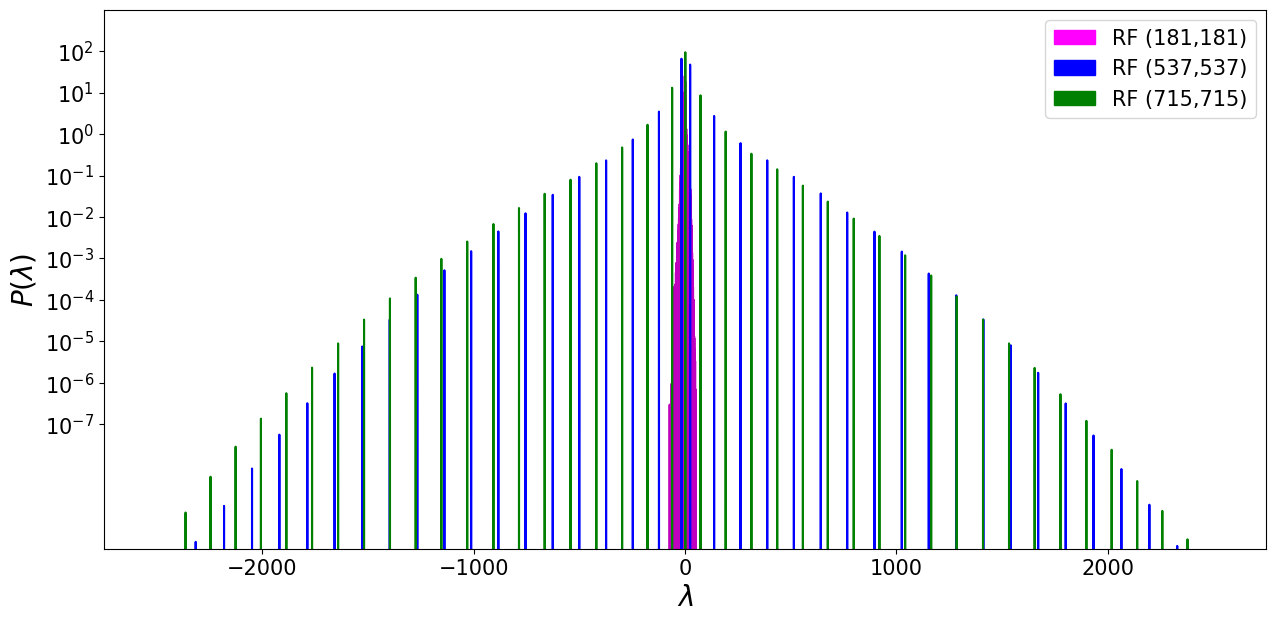
\includegraphics[width=7cm]{images/Hessian_spectre_vgg19_init_cifar10.png}
    \caption{Before Training}
    \label{subfig:Hessian_VGG_before_training}
     \end{subfigure}
      \hfill
     \begin{subfigure}[b]{0.45\textwidth}
    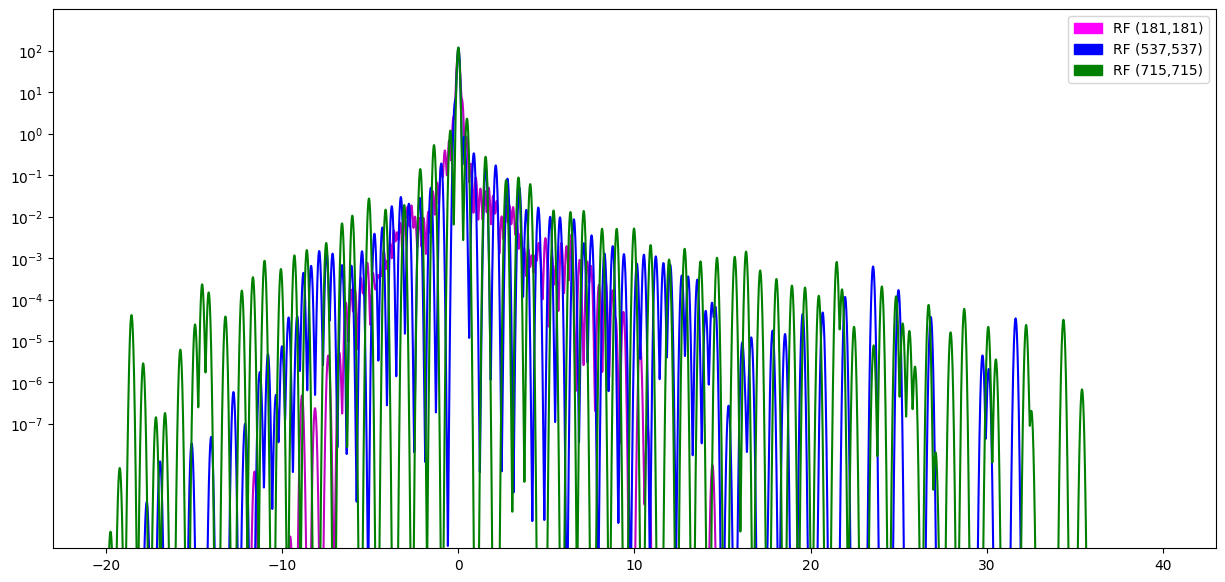
\includegraphics[width=7cm]{images/Hessian_spectre_vgg19_trained_cifar10.png}
    \caption{After training}
    \label{subfig:Hessian_VGG_after_training}
     \end{subfigure}
     \caption{Largest 90 eigen values of VGG model on CIFAR10 for different Receptive Fields \todo[inline]{Here I can
         put labels
     like $\lambda$ and $P(\lambda)$. Larger font} }
    \label{fig:hessian_vgg_cifar10}
\end{figure}
\begin{figure}[h]
 \centering
     \begin{subfigure}[b]{0.45\textwidth}
    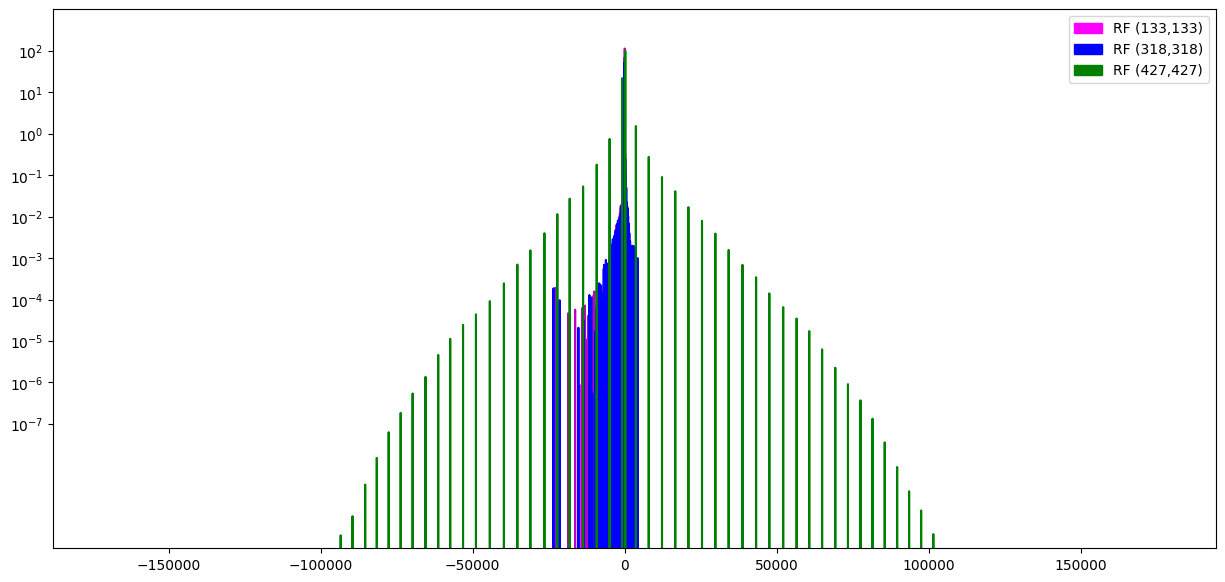
\includegraphics[width=7cm]{images/Hessian_spectre_resnet50_init_cifar10.png}
    \caption{Before Training}
    \label{subfig:}
     \end{subfigure}
      \hfill
     \begin{subfigure}[b]{0.45\textwidth}
    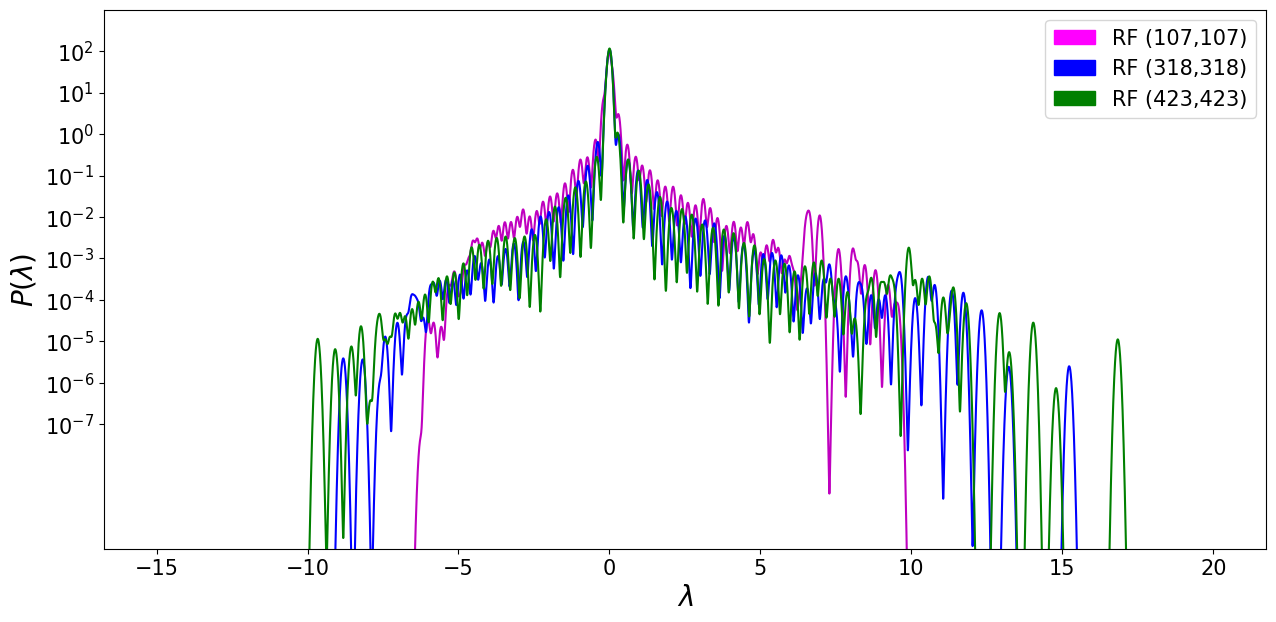
\includegraphics[width=7cm]{images/Hessian_spectre_resnet50_trained_cifar10.png}
    \caption{After training}
    \label{subfig:}
     \end{subfigure}
     \caption{Largest 90 eigen values of ResNet50 model on CIFAR10 for different Receptive Fields }
    \label{fig:hessian_resnet50_cifar10}
\end{figure}

But how does this affect the features or representations that these models learn? Next we show the similarity of the
internal representation two different seeds of the ReseNet50 model on CIFAR10., It is observed that the introduction of
larger receptive fields results in a divergence of representations within the deepest layers. This phenomenon can be
attributed to the heightened "chaotic" nature of the loss landscape, as indicated by the Hessian spectra in \Cref{fig:hessian_resnet50_cifar10}, particularly in instances where larger receptive fields are employed. Notably, the
representations in deeper layers for individual seeds exhibit dissimilarity, as they tend to converge into distinct
basins, differing not only from the majority of the network but also from corresponding layers in other seeds. The representation
 similarly was calculated using the first 1000 images of the test set and we use the Centred linear Kernel Alignment
 \citep{kornblithSimilarityNeuralNetwork2019} as similarity measure.
\begin{figure}[H]
        \centering
        \begin{subfigure}[b]{0.475\textwidth}
            \centering
            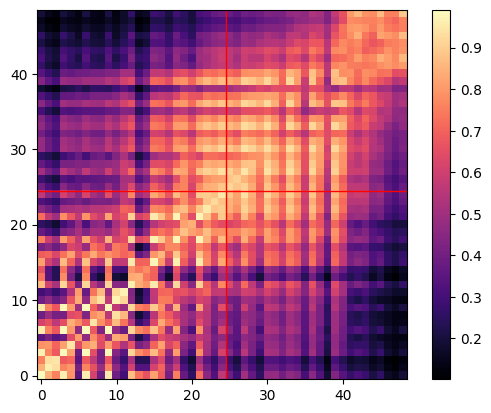
\includegraphics[width=0.7\textwidth]{images/resnet50_level1_similarity_cifar10.png}
            \caption[Network1]%
            {{\small Receptive field 110}}    
            \label{fig:similarity_lvl1}
        \end{subfigure}
        \hfill
        \begin{subfigure}[b]{0.475\textwidth}  
            \centering 
            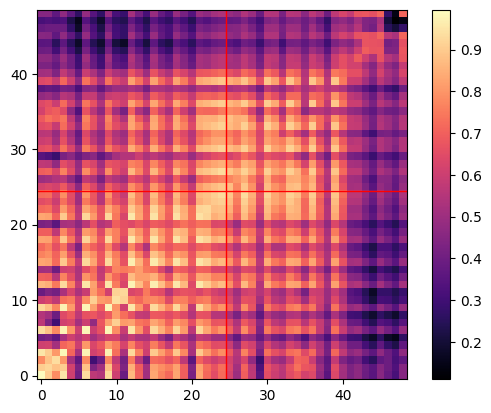
\includegraphics[width=0.7\textwidth]{images/resnet50_level2_similarity_cifar10.png}
            \caption[Network2]%
            {{\small Receptive field 213}}    
            \label{fig:similarity_lvl2}
        \end{subfigure}

        \vskip\baselineskip

        \begin{subfigure}[b]{0.475\textwidth}   
            \centering 
            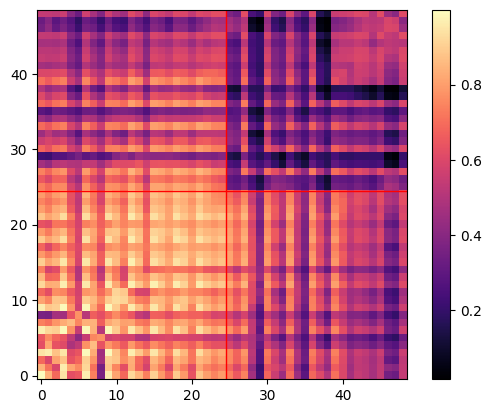
\includegraphics[width=0.7\textwidth]{images/resnet50_level3_similarity_cifar10.png}
            \caption[]%
            {{\small Receptive field 318}}    
            \label{fig:similarity_lvl3}
        \end{subfigure}
        \hfill
        \begin{subfigure}[b]{0.475\textwidth}   
            \centering 
            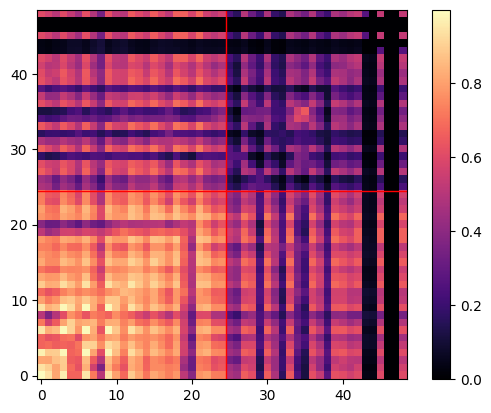
\includegraphics[width=0.7\textwidth]{images/resnet50_level4_similarity_cifar10.png}
            \caption[]%
            {{\small Receptive field 423}}    
            \label{fig:similarity_lvl4}
        \end{subfigure}
        \caption[ The average and standard deviation of critical parameters ]
        {\small Representation similarly of all layers in ReseNet50 for different receptive fields. The red lines
        represent the middle layer of the model (25$^{\textrm{th}}$ layer). The largest receptive field (bottom right)
      has high degree of dissimilarity between its deeper layer representations when compared with the smallest
    receptive field (top left)}
        \label{fig:similarity_resenet50}
    \end{figure}



\subsection{Receptive Field and Pixel Importance}\label{subsec:Receptive_field_and_pixel_importance}
In this section we show the projection of gradient of the last convolutional network into an input space of 64x64. We
show that for larger receptive fields the ``importance pattern'' does not change much but the ``importance'' decreases
from one receptive field to another. This means that even if the model sees similarity for all receptive fields, for
larger receptive fields each pixel is less important. We call importance here to the magnitude of the projected
gradient on the input space from the last convolutional layer of the  randomly initialised model. We place a would be gradient with 1 in the center of all channels
of the last convolutional layer and calculate the gradient with respect to a random input with 64x64 dimensions, we take
the absolute value of that projected gradient. Then for each receptive field we average 50 of such projections and also
take the average of their maximum value. In \Cref{fig:gradient_projection_resenet50,fig:gradient_projection_vgg} we can see the importance pattern for ReseNet50 and
VGG. In \Cref{fig:gradient_projection_vgg} the check board pattern appears due an odd-sized kernel is applied with an
even stride causing what \cite{kimDeadPixelTest2023} call \textit{pixel sensitivity imbalance}.
In \Cref{tab:vgg_grad_projection,tab:resnet50_grad_projection} can be seen the average of the maximum importance value for each receptive
field. As we can see the importance for each pixel is decreased as we increase the receptive field. This might explain
why having a larger receptive field could hinder performance, since we are paying attention to the same areas of the
image but not the same value of attention.

\begin{figure}[H]
        \centering
        \begin{subfigure}[b]{0.475\textwidth}
            \centering
            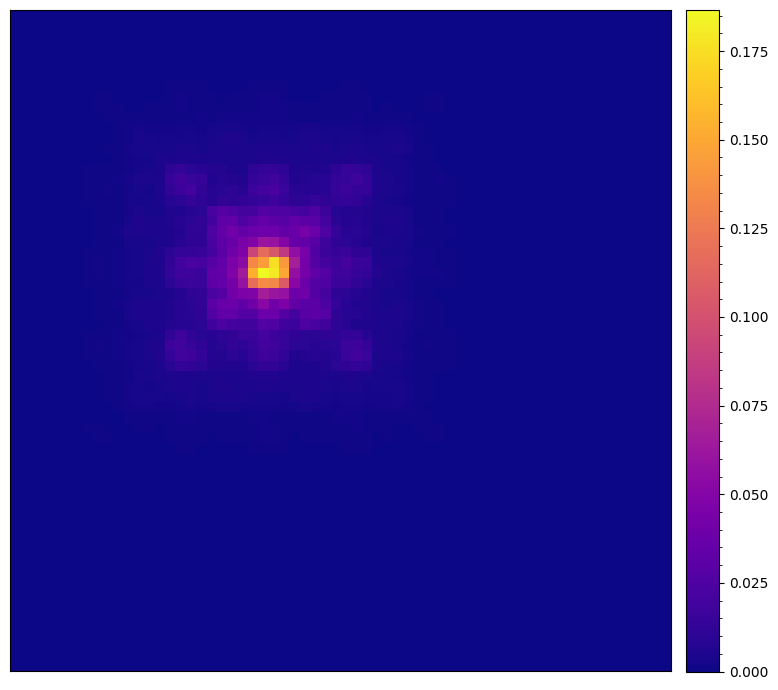
\includegraphics[width=0.7\textwidth]{images/gradientProjection_resnet_50_110.png}
            \caption[Network1]%
            {{\small Receptive field 110}}    
            \label{fig:similarity_lvl1}
        \end{subfigure}
        \hfill
        \begin{subfigure}[b]{0.475\textwidth}  
            \centering 
            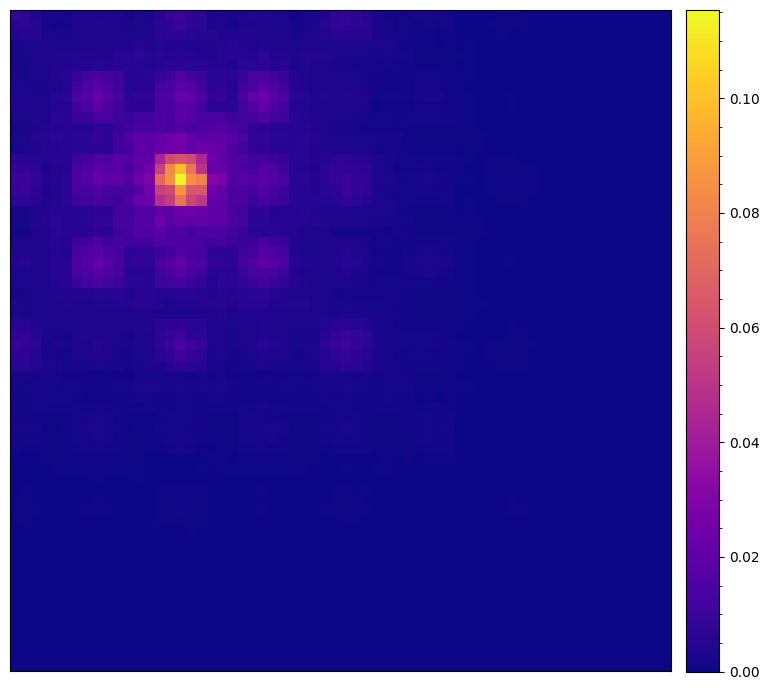
\includegraphics[width=0.7\textwidth]{images/gradientProjection_resnet_50_213.png}
            \caption[Network2]%
            {{\small Receptive field 213}}    
            \label{fig:similarity_lvl2}
        \end{subfigure}

        \vskip\baselineskip

        \begin{subfigure}[b]{0.475\textwidth}   
            \centering 
            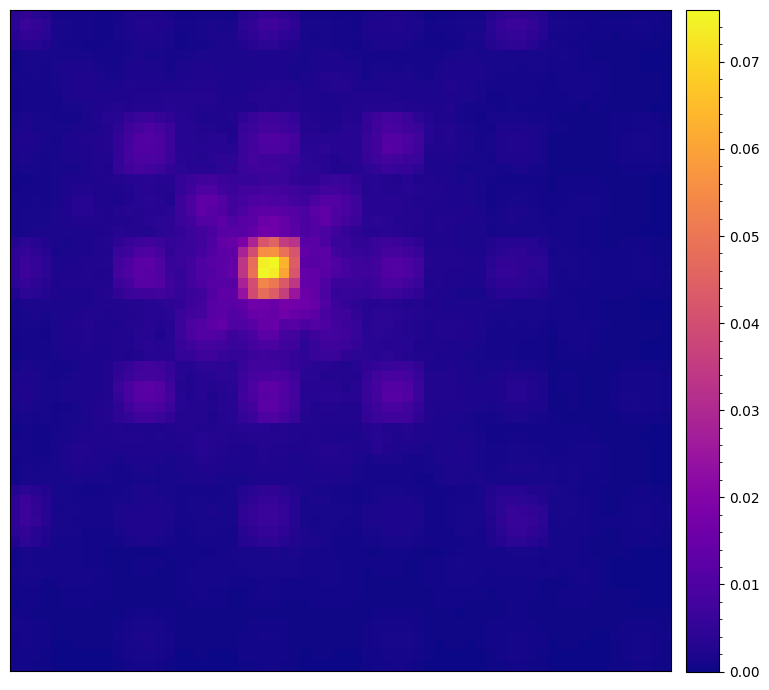
\includegraphics[width=0.7\textwidth]{images/gradientProjection_resnet_50_318.png}
            \caption[]%
            {{\small Receptive field 318}}    
            \label{fig:similarity_lvl3}
        \end{subfigure}
        \hfill
        \begin{subfigure}[b]{0.475\textwidth}   
            \centering 
            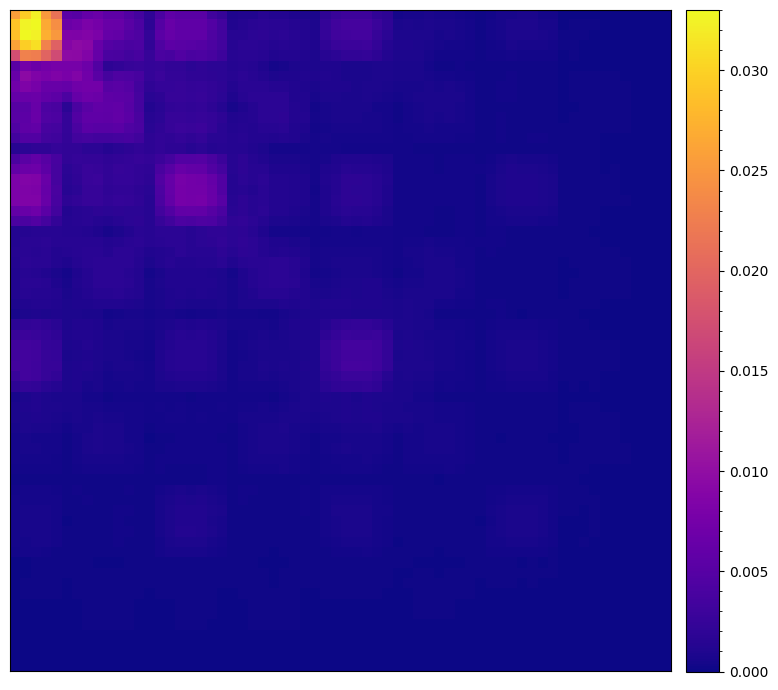
\includegraphics[width=0.7\textwidth]{images/gradientProjection_resnet_50_423.png}
            \caption[]%
            {{\small Receptive field 423}}    
            \label{fig:similarity_lvl4}
        \end{subfigure}
        \caption{\small Projection of the gradient into an input space of 64x64 for different levels of receptive field
        of ReseNet50}
        \label{fig:gradient_projection_resenet50}
    \end{figure}
\begin{figure}[H]
        \centering
        \begin{subfigure}[b]{0.475\textwidth}
            \centering
            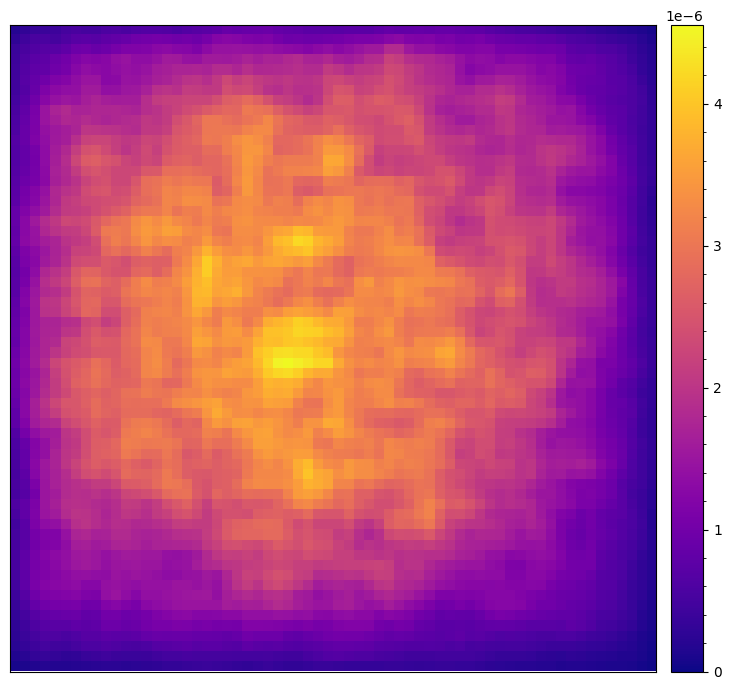
\includegraphics[width=0.7\textwidth]{images/gradientProjection_vgg19_1.png}
            \caption[Network1]%
            {{\small Receptive Field 181}}    
            \label{fig:grad_projection_vgg_lvl1}
        \end{subfigure}
        \hfill
        \begin{subfigure}[b]{0.475\textwidth}  
            \centering 
            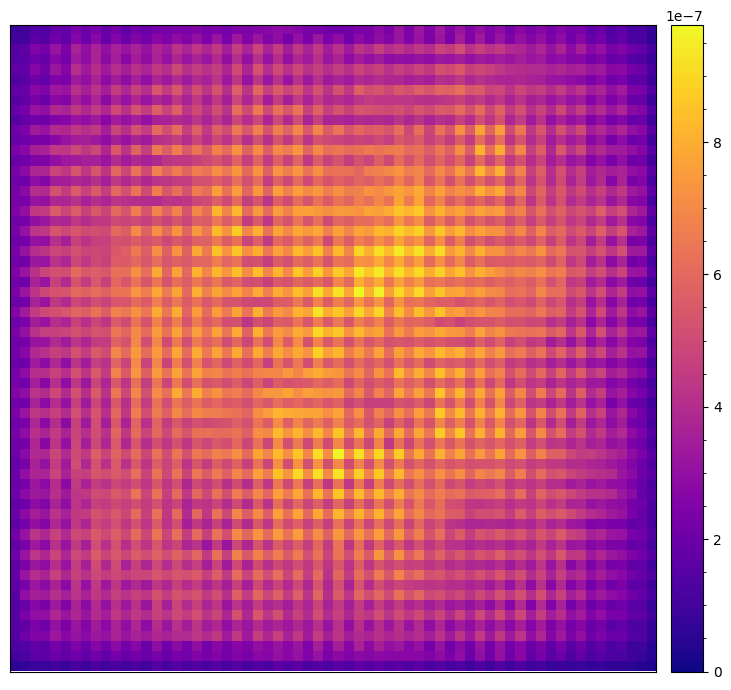
\includegraphics[width=0.7\textwidth]{images/gradientProjection_vgg19_2.png}
            \caption[Network2]%
            {{\small Receptive Field 359}}    
            \label{fig:grad_projection_vgg_lvl2}
        \end{subfigure}

        \vskip\baselineskip

        \begin{subfigure}[b]{0.475\textwidth}   
            \centering 
            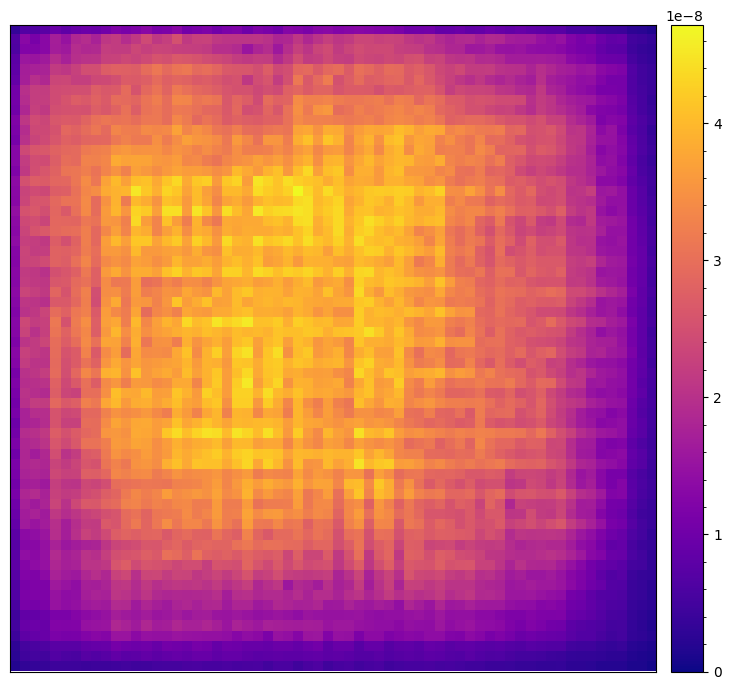
\includegraphics[width=0.7\textwidth]{images/gradientProjection_vgg19_3.png}
            \caption[]%
            {{\small Receptive Field 537}}    
            \label{fig:grad_projection_vgg_lvl3}
        \end{subfigure}
        \hfill
        \begin{subfigure}[b]{0.475\textwidth}   
            \centering 
            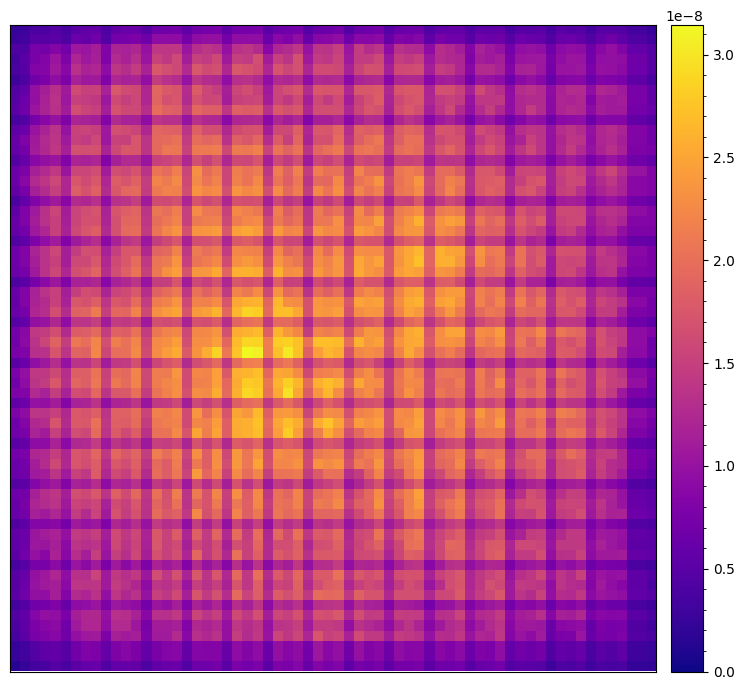
\includegraphics[width=0.7\textwidth]{images/gradientProjection_vgg19_4.png}
            \caption[]%
            {{\small Receptive Field 715}}    
            \label{fig:grad_projection_vgg_lvl4}
        \end{subfigure}
        \caption{\small Projection of the gradient into an input space of 64x64 for different levels of receptive field
        of ReseNet50}
        \label{fig:gradient_projection_vgg}
    \end{figure}



\begin{table}[H]
\begin{tabular}{@{}cc@{}}
\toprule
\textbf{Receptive Field} & \textbf{Maximum Projected Gradient Value} \\ \midrule
181                      & 1.24e-05 $\pm$ 2.14e-06                   \\
359                      & 2.48e-06 $\pm$ 4.88e-07                   \\
537                      & 1.32e-07 $\pm$ 2.48e-08                   \\
715                      & 7.26e-08 $\pm$ 1.45e-08                   \\ \bottomrule
\end{tabular}
\caption{VGG gradient projection on a 64X64 input image}
\label{tab:vgg_grad_projection}
\end{table}
\begin{table}[H]
\begin{tabular}{@{}cc@{}}
\toprule
\textbf{Receptive Field} & \textbf{Maximum Projected Gradient Value} \\ \midrule
110                      & 0.322 $\pm$ 0.122                         \\
213                      & 0.179 $\pm$ 0.079                         \\
318                      & 0.111 $\pm$ 0.039                         \\
423                      & 0.064 $\pm$ 0.022                         \\ \bottomrule
\end{tabular}
\caption{Maximum projected gradient for ReseNet50}
\label{tab:resnet50_grad_projection}
\end{table}

%
%\subsection{}
%
%
%
%\begin{figure*}[!htb]
% \centering
%     \begin{subfigure}[b]{\columnwidth}
%    \includegraphics[width=1.1\columnwidth]{}
%    \caption{}
%    \label{}
%     \end{subfigure}
%      \hfill
%     \begin{subfigure}[b]{\columnwidth}
%    \includegraphics[width=1.1\columnwidth]{}
%    \caption{}
%    \label{}
%     \end{subfigure}
%     \caption{}
%    \label{}
%\end{figure*}
%
%





%
%\begin{figure}[ht]
%  \centering
%  \includegraphics[width=0.8\textwidth]{}
%  \caption{}
%  \label{fig:}
%\end{figure}

